%% =============================================================
%%  Les gammes — construction par tétracordes
%%  Guide de référence, composé en LaTeX, gravures LilyPond
%% =============================================================
%%
%%  Les figures (gravures/*.cropped.pdf) et les tableaux
%%  (gravures/*.tex) sont produits par outils/generer.py, qui les
%%  dérive d'un modèle de hauteurs unique — le même que celui des
%%  fichiers MusicXML. Voir le colophon en dernière page.
%%
\documentclass[a4paper,11pt]{article}

\usepackage[top=2.2cm,bottom=2.4cm,left=2.2cm,right=2.2cm]{geometry}
\usepackage[T1]{fontenc}
\usepackage[utf8]{inputenc}
\usepackage[french]{babel}
\usepackage{lmodern}
\usepackage{xcolor}
\usepackage{graphicx}
\usepackage{titlesec}
\usepackage{fancyhdr}
\usepackage{mdframed}
\usepackage{array}
\usepackage{enumitem}
\usepackage{booktabs}
\usepackage{longtable}
\usepackage{hyperref}

\graphicspath{{gravures/}}

% ---- Couleurs, reprises du document des accords de guitare ---------
\definecolor{navy}{RGB}{18,50,105}
\definecolor{lightnavy}{RGB}{235,241,255}
\definecolor{mygray}{RGB}{110,110,110}
\definecolor{accent}{RGB}{150,40,30}

\hypersetup{colorlinks=true, linkcolor=navy, urlcolor=navy,
  pdftitle={Les gammes — construction par tétracordes},
  pdfauthor={Fabian Bastin}}

% ---- En-tête et pied -----------------------------------------------
\pagestyle{fancy}
\fancyhf{}
\renewcommand{\headrulewidth}{0.4pt}
\renewcommand{\footrulewidth}{0.4pt}
\fancyhead[L]{\small\bfseries\textcolor{navy}{Les gammes}}
\fancyhead[R]{\small\textcolor{mygray}{\thepage}}
\fancyfoot[C]{\small\textcolor{mygray}{Construction par tétracordes}}

% ---- Titres de section ---------------------------------------------
\newcommand{\navysect}[1]{%
  \colorbox{navy}{%
    \parbox[c][17pt]{\dimexpr\linewidth-2\fboxsep\relax}{%
      \color{white}\hspace{6pt}\bfseries\normalsize #1}}%
}
\titleformat{\section}[block]{\normalfont}{}{0pt}{\navysect}
\titlespacing*{\section}{0pt}{16pt}{10pt}
\titleformat{\subsection}
  {\normalfont\normalsize\bfseries\color{navy}}{\thesubsection}{0.6em}{}
\titlespacing*{\subsection}{0pt}{12pt}{5pt}

% ---- Encadré de remarque -------------------------------------------
\newmdenv[linecolor=navy, linewidth=0.5pt, backgroundcolor=lightnavy,
  innertopmargin=6pt, innerbottommargin=6pt,
  innerleftmargin=8pt, innerrightmargin=8pt,
  skipabove=8pt, skipbelow=8pt]{remarque}

% ---- Figure gravée ---------------------------------------------------
% Les gravures sont rognées au trait par LilyPond ; on les centre sans
% cadre, avec une légende discrète.
\newcommand{\gravure}[2]{%
  \begin{center}
    \includegraphics[max width=\linewidth]{#1.cropped.pdf}\\[2pt]
    {\small\itshape\color{mygray} #2}
  \end{center}%
}

% `max width` vient de adjustbox ; à défaut, on se rabat sur width.
\usepackage[export]{adjustbox}

% ---- Gamme de référence, pour les planches finales -------------------
% Les gravures de référence sortent toutes à 224 pt de large (largeur de ligne
% fixée côté LilyPond), si bien que `width` leur applique à toutes le même
% facteur d'échelle. Avec des largeurs naturelles disparates — elles allaient de
% 154 à 202 pt selon l'encombrement de l'armure — la même commande aurait donné
% des portées de tailles différentes sur une même page.
\newcommand{\gammeref}[2]{%
  \parbox[t]{0.48\linewidth}{%
    \small\textbf{\color{navy}#2}\\[2pt]
    \includegraphics[width=\linewidth]{#1.cropped.pdf}\\[6pt]}%
  \hfill}

\setlist{itemsep=2pt, topsep=4pt, parsep=0pt}

\begin{document}

% =====================================================================
\begin{titlepage}
\centering
\vspace*{3cm}
{\Huge\bfseries\color{navy} Les gammes\par}
\vspace{0.6cm}
{\LARGE\color{navy} Construction par tétracordes\par}
\vspace{1.4cm}
{\large Majeures, mineures naturelles, harmoniques et mélodiques\par}
\vspace{0.4cm}
{\large Les quinze tonalités\par}
\vspace{2.5cm}
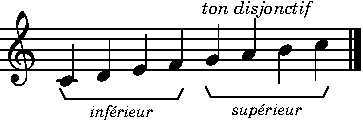
\includegraphics[width=0.62\linewidth]{f-do-majeur.cropped.pdf}
\vfill
{\small\color{mygray}
Gravures LilyPond, composition \LaTeX.\\
Fichiers MusicXML joints.\par}
\vspace{1cm}
\end{titlepage}

\tableofcontents
\newpage

% =====================================================================
\section{Avant-propos}

Ce guide explique comment les gammes se construisent, plutôt que de les
énumérer. Le fil conducteur est le \emph{tétracorde} : un groupe de quatre
notes qui, répété et transposé, engendre la gamme majeure, explique le cycle
des quintes et rend les trois gammes mineures comparables entre elles.

C'est le second de deux guides. Il emploie les intervalles — seconde,
tierce, quarte juste, triton, seconde augmentée — sans les redéfinir : leur
construction, un numéro compté en lettres et une qualité comptée en
demi-tons, fait l'objet du premier,
\href{https://www.slashbin.net/musique/theorie/intervalles.pdf}{\emph{Les
intervalles — du demi-ton à l'octave}}, qu'il vaut mieux lire d'abord.

L'approche a un avantage pratique. Retenir sept intervalles par gamme et
quatre familles de gammes fait vingt-huit choses à mémoriser ; retenir quatre
tétracordes et la règle qui les assemble en fait cinq. Les tableaux de la
section~\ref{sec:reference} restent disponibles pour vérifier, mais ils
devraient devenir superflus.

\begin{remarque}
\textbf{Conventions.} Les hauteurs sont nommées en français
(\emph{do, ré, mi, fa, sol, la, si}). Le demi-ton est le plus petit
intervalle du système tempéré ; le ton en vaut deux. Les degrés d'une gamme
sont numérotés de 1 à 7 à partir de la tonique.
\end{remarque}

Les fichiers \texttt{MusicXML} qui accompagnent ce document contiennent les
soixante gammes, lisibles par MuseScore, Finale, Sibelius ou tout autre
éditeur de partitions. La section~\ref{sec:musicxml} explique ce qu'ils
contiennent.

% =====================================================================
\section{Le matériau : tons et demi-tons}
\label{sec:materiau}

L'octave tempérée se divise en douze demi-tons égaux. La notation, elle,
ne dispose que de \emph{sept} lettres — do, ré, mi, fa, sol, la, si — qu'il
faut donc altérer pour atteindre les cinq hauteurs restantes.

Ce décalage entre douze sons et sept noms n'est pas un défaut : c'est lui qui
permet d'écrire une gamme. Une gamme heptatonique emploie chaque lettre
\emph{une fois et une seule}. C'est la raison pour laquelle on écrit
\emph{fa dièse} en sol majeur et jamais \emph{sol bémol}, bien que les deux
sonnent identiquement sur un piano : la lettre \emph{sol} est déjà prise par
le cinquième degré.

Parmi les gammes de sept notes, une disposition a reçu un nom : la gamme
\textbf{diatonique}, du grec \emph{diatonikos}, « à travers les tons ». Elle
compte \emph{cinq tons et deux demi-tons}, et ses deux demi-tons sont aussi
éloignés l'un de l'autre que possible : deux tons les séparent d'un côté,
trois de l'autre. Les touches blanches du piano en sont l'exemple type — les
deux demi-tons mi--fa et si--do y sont séparés par deux tons (do--ré--mi) et
par trois (fa--sol--la--si). À l'opposé, la gamme \textbf{chromatique}
avance par les douze demi-tons de l'octave ; elle a plus de notes que de
lettres, et doit donc en répéter.

\begin{remarque}
Cette règle a une conséquence que l'on rencontre plus loin : certaines
gammes exigent des \emph{doubles dièses}. En ré dièse mineur harmonique, le
septième degré s'écrit \emph{do double dièse} — et non \emph{ré}, déjà
occupé par la tonique.
\end{remarque}

% =====================================================================
\section{Le tétracorde}

Un \textbf{tétracorde} est un groupe de quatre notes conjointes couvrant une
quarte juste, soit cinq demi-tons. Trois intervalles suffisent donc à le
décrire entièrement. Le mot vient du grec \emph{tetrachordon}, « quatre
cordes » : c'est l'unité de base de la théorie grecque, dont la nôtre
descend.

Quatre types suffisent pour tout ce qui suit.

\begin{center}
%% Produit par outils/generer.py — ne pas modifier à la main.

\begin{tabular}{@{}l l l@{}}
\toprule
\textbf{Tétracorde} & \textbf{Intervalles} & \textbf{Exemple sur do} \\
\midrule
majeur & ton -- ton -- ½ ton & do -- ré -- mi -- fa \\
mineur & ton -- ½ ton -- ton & do -- ré -- mi bémol -- fa \\
phrygien & ½ ton -- ton -- ton & do -- ré bémol -- mi bémol -- fa \\
harmonique & ½ ton -- 1 ½ ton -- ½ ton & do -- ré bémol -- mi -- fa \\
lydien & ton -- ton -- ton & do -- ré -- mi -- fa dièse \\
\bottomrule
\end{tabular}



\end{center}

\gravure{f-quatre-tetracordes}{Les quatre tétracordes, tous à partir de do.}

Le tétracorde \emph{lydien} figure dans le tableau pour mémoire : couvrant
un triton et non une quarte juste, il ne sert pas à l'assemblage décrit ici.

% =====================================================================
\section{La gamme majeure}

\subsection{Deux tétracordes et un ton}

\textbf{Une gamme majeure est faite de deux tétracordes majeurs, séparés par
un ton.} Ce ton n'appartient à aucun des deux ; on l'appelle
\emph{ton disjonctif}.

\gravure{f-do-majeur}{Do majeur : deux tétracordes majeurs identiques,
séparés par le ton disjonctif fa--sol.}

Les deux tétracordes sont \emph{identiques} en intervalles : ton, ton,
demi-ton. La gamme majeure est donc une structure symétrique, ce que sa suite
d'intervalles — ton, ton, demi-ton, \textbf{ton}, ton, ton, demi-ton — cache
plutôt qu'elle ne le montre. Vue ainsi, la position des deux demi-tons n'est
plus à mémoriser : ils tombent nécessairement entre les degrés 3 et 4, et
entre les degrés 7 et 8, parce que chaque tétracorde finit par un demi-ton.

Entre ces deux demi-tons, on compte deux tons d'un côté (du degré 1 au
degré 3) et trois de l'autre (du degré 4 au degré 7) : c'est exactement la
disposition diatonique de la section~\ref{sec:materiau}. Le nom complet de la
gamme majeure est donc \textbf{gamme diatonique majeure} ; l'usage l'abrège
en « gamme majeure », et ce guide fait de même.

\subsection{Les degrés et leurs noms}
\label{sec:degres}

\gravure{f-degres}{Les sept degrés de do majeur et leur nom français.}

Chaque degré porte un nom qui décrit sa fonction, non sa hauteur :

\begin{itemize}
  \item \textbf{tonique} (1) — le centre de gravité, celui sur lequel la
    gamme se repose ;
  \item \textbf{sus-tonique} (2) — au-dessus de la tonique ;
  \item \textbf{médiante} (3) — à mi-chemin entre tonique et dominante ;
    c'est elle qui décide du caractère majeur ou mineur ;
  \item \textbf{sous-dominante} (4) — une quinte \emph{au-dessous} de la
    tonique, et non « sous la dominante » comme le nom le suggère ;
  \item \textbf{dominante} (5) — le degré le plus fort après la tonique ;
  \item \textbf{sus-dominante} (6) — au-dessus de la dominante ;
  \item \textbf{sensible} (7) — à un demi-ton sous la tonique, vers laquelle
    elle attire l'oreille.
\end{itemize}

\begin{remarque}
\textbf{Sensible ou sous-tonique ?} Le septième degré ne s'appelle
\emph{sensible} que s'il se trouve à un \emph{demi-ton} de la tonique. S'il
en est à un ton entier — ce qui arrive en mineur naturel — on parle de
\textbf{sous-tonique}, et l'attraction vers la tonique disparaît. Cette
distinction, propre à la terminologie française, explique à elle seule
l'existence de la gamme mineure harmonique (section~\ref{sec:mineures}).
\end{remarque}

% =====================================================================
\section{Le cycle des quintes, conséquence du tétracorde}

\subsection{Le mécanisme}
\label{sec:mecanisme}

Voici l'observation qui fait tout le reste :

\begin{remarque}
\textbf{Le tétracorde supérieur d'une gamme majeure est le tétracorde
inférieur de la gamme située une quinte au-dessus.}
\end{remarque}

Le tétracorde supérieur de do majeur est \emph{sol--la--si--do}. Or c'est
exactement le tétracorde inférieur de sol majeur. Il ne reste qu'à lui
adjoindre un tétracorde majeur à partir de ré — \emph{ré--mi--fa dièse--sol} —
et la gamme de sol majeur est complète.

\gravure{f-chaine-quintes}{Le tétracorde supérieur de do majeur devient le
tétracorde inférieur de sol majeur. Le fa dièse n'est pas un choix : il est
imposé par la structure du tétracorde.}

Le fa dièse n'a pas été décidé. Il est \emph{exigé} : sans lui, le second
tétracorde de sol majeur serait ré--mi--fa--sol, c'est-à-dire un tétracorde
mineur, et la gamme ne serait plus majeure. Chaque quinte ascendante ajoute
ainsi exactement une altération, et toujours la même.

Un tétracorde majeur appartient donc à deux gammes majeures, et ses notes
extrêmes suffisent à les nommer :

\begin{remarque}
\textbf{Un tétracorde majeur est le tétracorde inférieur de la gamme de sa
première note, et le tétracorde supérieur de la gamme de sa dernière note.}
Ainsi \emph{sol--la--si--do} ouvre sol majeur et achève do majeur.
\end{remarque}

Il n'apparaît dans aucune autre gamme majeure. Les seules quatre notes
conjointes d'une gamme majeure qui s'enchaînent par ton, ton, demi-ton sont
les degrés 1 à 4 et 5 à 8 ; ailleurs, le demi-ton tombe à une autre place, ou
manque, comme entre les degrés 4 et 7, séparés par trois tons.

\subsection{L'ordre des altérations}

En montant de quinte en quinte à partir de do, les dièses apparaissent dans
un ordre fixe :

\begin{center}
\textbf{fa\ \ do\ \ sol\ \ ré\ \ la\ \ mi\ \ si}
\end{center}

En descendant de quinte en quinte — ce qui revient à monter de quarte — ce
sont les bémols, dans l'ordre exactement inverse :

\begin{center}
\textbf{si\ \ mi\ \ la\ \ ré\ \ sol\ \ do\ \ fa}
\end{center}

Ces deux suites n'ont pas à être apprises : elles se \emph{démontrent}. Il
suffit d'appliquer le mécanisme de la section~\ref{sec:mecanisme} de proche
en proche, à partir de do majeur, dans un sens pour les dièses et dans
l'autre pour les bémols.

Les deux chaînes sont gravées ci-dessous, une gamme par ligne, chacune avec
son armure. Le signe que la construction vient d'ajouter à l'armure est en
couleur, comme la note qu'il affecte.

\begin{center}
\begin{minipage}[t]{0.49\linewidth}
  \centering
  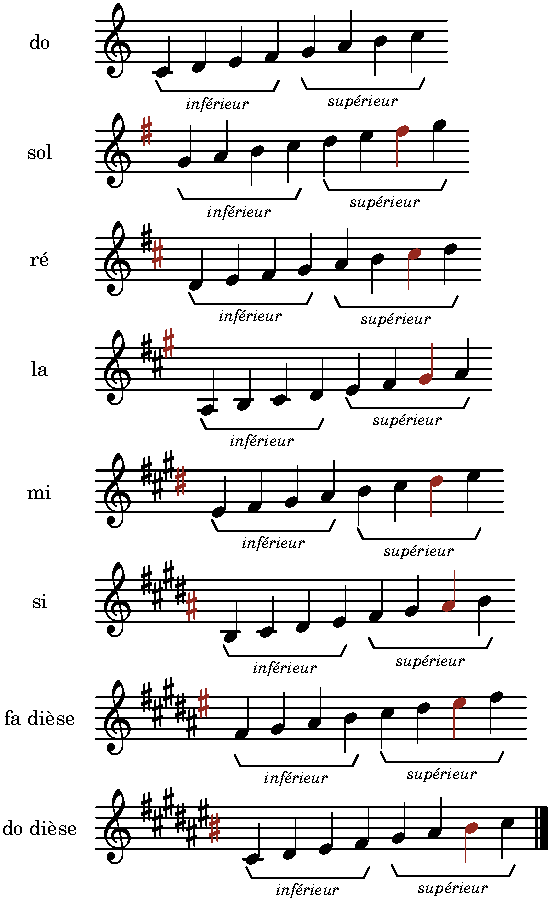
\includegraphics[width=\linewidth]{f-chaine-dieses.cropped.pdf}\\[2pt]
  {\small\itshape\color{mygray} Vers les dièses : le supérieur devient
  l'inférieur.}
\end{minipage}\hfill
\begin{minipage}[t]{0.49\linewidth}
  \centering
  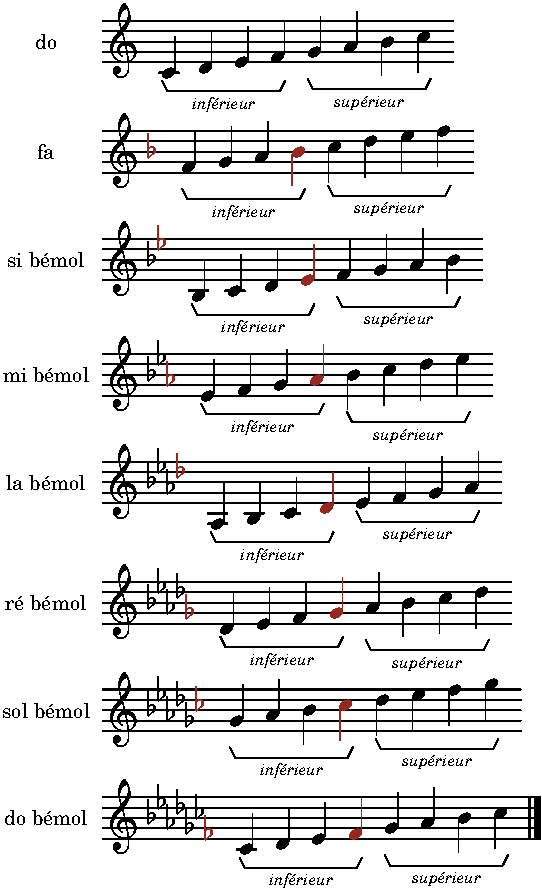
\includegraphics[width=\linewidth]{f-chaine-bemols.cropped.pdf}\\[2pt]
  {\small\itshape\color{mygray} Vers les bémols : l'inférieur devient le
  supérieur.}
\end{minipage}
\end{center}

\paragraph{Les dièses : le tétracorde supérieur devient l'inférieur.}
On garde le tétracorde supérieur d'une gamme majeure et on en fait le
tétracorde inférieur de la suivante, dont la tonique est l'ancienne
dominante, une quinte plus haut. Il reste à bâtir le nouveau tétracorde
supérieur, un ton disjonctif plus haut.

Sur la figure de gauche, chaque tétracorde supérieur d'une portée se
retrouve comme tétracorde inférieur de la portée suivante, sans rien y
changer. Le tétracorde à bâtir
reprend, lui, les lettres des degrés 2 à 5 de l'ancienne gamme — ré, mi, fa,
sol en partant de do. Dans l'ancienne gamme, ces quatre notes sont séparées
par un ton, un demi-ton, puis un ton : c'est un tétracorde \emph{mineur}.
Pour le rendre majeur (ton, ton, demi-ton), une seule correction est
possible : \textbf{hausser sa troisième note d'un demi-ton}. Cette note était
la sous-dominante de l'ancienne gamme ; elle devient la \emph{sensible} de
la nouvelle.

Chaque étape ajoute donc exactement un dièse. Comme chaque tonique est une
quinte au-dessus de la précédente, chaque nouvelle sensible l'est aussi, et
les dièses s'enchaînent de quinte en quinte : fa, do, sol, ré, la, mi, si.

\paragraph{Les bémols : le tétracorde inférieur devient le supérieur.}
On fait l'opération inverse. Le tétracorde inférieur d'une gamme majeure
devient le tétracorde supérieur de la suivante, dont la tonique est
l'ancienne sous-dominante, une quinte plus bas. Il reste à bâtir le nouveau
tétracorde inférieur, un ton disjonctif plus bas. Sur la figure de droite,
chaque tétracorde inférieur d'une portée se retrouve comme tétracorde
supérieur de la portée suivante.

Le tétracorde à bâtir reprend les lettres des degrés 4 à 7 de l'ancienne
gamme — fa, sol, la, si en partant de do. Ces quatre notes sont séparées par
trois tons : c'est le tétracorde \emph{lydien}, qui couvre un triton au lieu
d'une quarte juste. Là encore, une seule correction est possible :
\textbf{abaisser sa quatrième note d'un demi-ton}. Cette note était la
sensible de l'ancienne gamme ; elle devient la \emph{sous-dominante} de la
nouvelle. Du même coup, le demi-ton qui la séparait de l'ancienne tonique
s'élargit en ton : c'est le nouveau ton disjonctif.

Chaque étape ajoute donc exactement un bémol. Chaque tonique est une quinte
au-dessous de la précédente, et les bémols s'enchaînent de quinte en quinte
descendante : si, mi, la, ré, sol, do, fa.

\begin{remarque}
\textbf{Deux règles pratiques en découlent.} Le dernier dièse de l'armure
est la \emph{sensible} de la tonalité : un demi-ton au-dessus, on trouve la
tonique. Le dernier bémol de l'armure est sa \emph{sous-dominante} : une
quarte au-dessous, on trouve la tonique — c'est aussi l'avant-dernier bémol.
La section~\ref{sec:armure} en tire le relatif mineur et le moyen de trancher
entre majeur et mineur.
\end{remarque}

Les deux procédés sont exactement inverses : l'un fait du tétracorde
supérieur un tétracorde inférieur, l'autre du tétracorde inférieur un
tétracorde supérieur ; l'un hausse la note qui corrige un tétracorde mineur,
l'autre abaisse celle qui corrige un tétracorde lydien. Il n'est donc pas surprenant que les deux ordres soient l'un le
miroir de l'autre.

Les deux séries s'arrêtent au bout de sept étapes, quand les sept lettres
sont altérées. Une huitième étape — sol dièse majeur, ou fa bémol majeur —
exigerait un double dièse (fa double dièse) ou un double bémol (si double
bémol), qu'une armure ne contient jamais.

\subsection{Enharmonies}

Aux extrémités du cycle, trois paires de tonalités désignent les mêmes sons
sous deux écritures différentes :

\begin{center}
\begin{tabular}{@{}l c l@{}}
\toprule
\textbf{Écriture en dièses} & & \textbf{Écriture en bémols} \\
\midrule
si majeur (5 dièses) & = & do bémol majeur (7 bémols) \\
fa dièse majeur (6 dièses) & = & sol bémol majeur (6 bémols) \\
do dièse majeur (7 dièses) & = & ré bémol majeur (5 bémols) \\
\bottomrule
\end{tabular}
\end{center}

Le choix entre les deux relève de la commodité de lecture et du contexte
harmonique, non du son : on préfère l'armure la plus légère, sauf si la
tonalité voisine impose l'autre.

% =====================================================================
\section{Les gammes mineures}
\label{sec:mineures}

\subsection{La mineure naturelle, ou relative}

À toute gamme majeure correspond une gamme mineure qui emploie exactement les
mêmes notes, mais prend pour tonique son \emph{sixième degré}. À do majeur
répond la mineur ; l'armure est la même, le centre de gravité a changé.

En tétracordes, la mineure naturelle se lit : tétracorde \emph{mineur}, ton
disjonctif, tétracorde \emph{phrygien}.

Puisqu'elle a les notes d'une gamme majeure, elle en a aussi les cinq tons
et les deux demi-tons, disposés de la même façon : c'est la \textbf{gamme
diatonique mineure}. Les deux formes qui suivent la modifient, et cessent
par là d'être diatoniques au sens strict.

\subsection{La mineure harmonique}

La mineure naturelle a un défaut, et il est harmonique. Son septième degré
est à un \emph{ton} de la tonique : c'est une sous-tonique, pas une sensible.
L'attraction vers la tonique disparaît, et l'accord bâti sur la dominante
devient mineur — en la mineur, mi--sol--si au lieu de mi--sol dièse--si. La
cadence parfaite, qui fait reposer une phrase, perd sa force.

La solution est directe : on hausse le septième degré d'un demi-ton. La
sensible réapparaît, l'accord de dominante redevient majeur, la cadence
retrouve son effet. C'est de cet usage harmonique que la gamme tire son nom.

Le prix à payer se voit entre les degrés 6 et 7 :

\gravure{f-seconde-augmentee}{La mineure harmonique de la : entre fa et
sol dièse s'ouvre une seconde augmentée — un ton et demi entre deux degrés
voisins.}

Cet intervalle d'un ton et demi entre deux notes conjointes est la
signature sonore de la gamme. Il donne son caractère à une bonne part de la
musique d'Europe de l'Est et du Moyen-Orient — et il est réputé malcommode
à chanter.

\subsection{La mineure mélodique}

D'où la troisième forme : pour effacer la seconde augmentée, on hausse aussi
le \emph{sixième} degré. La montée devient régulière. À la descente, la
sensible n'a plus de rôle — rien n'attire vers une tonique qu'on quitte — et
l'on revient à la forme naturelle.

\gravure{f-la-mineures}{Les trois formes de la mineure de la : naturelle,
harmonique, mélodique ascendante.}

\begin{remarque}
En jazz, la forme ascendante s'emploie dans les deux sens ; on la nomme
alors \emph{mineure mélodique réelle}. Ce n'est pas une gamme différente,
c'est un usage différent de la même.
\end{remarque}

\subsection{Les quatre gammes en un tableau}

C'est ici que le détour par les tétracordes se rentabilise. Les quatre
gammes ne diffèrent que par leur tétracorde \emph{supérieur} — le tétracorde
inférieur est majeur pour la majeure, mineur pour les trois mineures, et
c'est tout.

\begin{center}
%% Produit par outils/generer.py — ne pas modifier à la main.

\begin{tabular}{@{}l l l@{}}
\toprule
\textbf{Gamme} & \textbf{Tétracorde inférieur} & \textbf{Tétracorde supérieur} \\
\midrule
majeure & majeur & majeur \\
mineure naturelle & mineur & phrygien \\
mineure harmonique & mineur & harmonique \\
mineure mélodique & mineur & majeur \\
\bottomrule
\end{tabular}


\end{center}

Le fait remarquable est la dernière ligne : \textbf{la mineure mélodique
ascendante est faite d'un tétracorde mineur et d'un tétracorde majeur}. Elle
est donc, littéralement, à mi-chemin entre la mineure naturelle et la
majeure — ce que son usage confirme.

\begin{remarque}
\textbf{Lesquelles sont diatoniques ?} Au sens strict — cinq tons et deux
demi-tons aussi éloignés que possible —, seules la majeure et la mineure
naturelle le sont. La mineure harmonique contient une seconde augmentée,
qui n'est ni un ton ni un demi-ton. La mineure mélodique ascendante a bien
cinq tons et deux demi-tons, mais mal répartis : entre les degrés 2--3 et
7--8, quatre tons d'un côté, un seul de l'autre. Beaucoup de manuels
emploient toutefois \emph{diatonique} au sens large, pour toute gamme de
sept notes conjointes qui prend chaque lettre une fois, par opposition à
\emph{chromatique} ; en ce sens, les trois mineures sont diatoniques.
\end{remarque}

% =====================================================================
\section{Lire une armure}
\label{sec:armure}

Une armure ne désigne pas une tonalité, mais deux : une majeure et sa relative
mineure, qui emploient les mêmes notes. Les retrouver demande trois règles, et
trancher entre les deux demande de regarder la partition. Aucune de ces règles
n'est à apprendre telle quelle : toutes découlent de la construction par
tétracordes.

\subsection{Avec des dièses : le dernier dièse est la sensible}

\begin{remarque}
\textbf{Le dernier dièse de l'armure est la sensible de la tonalité majeure.}
La tonique se trouve donc un demi-ton au-dessus du dernier dièse, sur la
lettre suivante.
\end{remarque}

Les dièses s'écrivent toujours dans le même ordre : fa, do, sol, ré, la, mi,
si. Il suffit de repérer le dernier, le plus à droite, et de monter d'un
demi-ton.

\begin{center}
%% Produit par outils/generer.py — ne pas modifier à la main.

\begin{tabular}{@{}l l l l l@{}}
\toprule
\textbf{Armure} & \textbf{\shortstack[l]{Dernier\\dièse}} & \textbf{\shortstack[l]{Tonique\\majeure}} & \textbf{\shortstack[l]{Relatif\\mineur}} & \textbf{\shortstack[l]{Sensible\\du mineur}} \\
\midrule
1~dièse & fa dièse & sol & mi & ré dièse \\
2~dièses & do dièse & ré & si & la dièse \\
3~dièses & sol dièse & la & fa dièse & mi dièse \\
4~dièses & ré dièse & mi & do dièse & si dièse \\
5~dièses & la dièse & si & sol dièse & fa double dièse \\
6~dièses & mi dièse & fa dièse & ré dièse & do double dièse \\
7~dièses & si dièse & do dièse & la dièse & sol double dièse \\
\bottomrule
\end{tabular}


\end{center}

\paragraph{Pourquoi.} Trois faits établis plus haut suffisent.
\begin{enumerate}
  \item Chaque quinte ascendante garde tous les dièses de la gamme précédente
    et en ajoute exactement un (section~\ref{sec:mecanisme}). Ce nouveau dièse
    est celui de la note qu'il faut hausser pour que le nouveau tétracorde
    supérieur soit majeur : sa troisième note, c'est-à-dire le septième degré
    de la gamme, sa \emph{sensible}.
  \item L'armure écrit les dièses dans l'ordre où le cycle les ajoute. Le plus
    à droite est donc le dernier ajouté : la sensible.
  \item La sensible est à un demi-ton sous la tonique
    (section~\ref{sec:degres}). Et comme une gamme emploie chaque lettre une
    fois et une seule, la tonique porte nécessairement la lettre qui suit celle
    de la sensible.
\end{enumerate}

Le troisième point évite un piège à six dièses. Le dernier est mi dièse, et la
tonique est \emph{fa dièse}, pas fa : fa sonne comme mi dièse (c'est la même
touche du piano), si bien que le demi-ton au-dessus de mi dièse est fa dièse.
Compter sur la lettre suivante règle la question sans y penser.

\subsection{Le relatif mineur : un ton sous le dernier dièse}

La relative mineure prend pour tonique le sixième degré de la gamme majeure
(section~\ref{sec:mineures}). Or le tétracorde supérieur d'une gamme majeure
finit par un ton puis un demi-ton : le sixième degré est un ton sous le
septième, qui est un demi-ton sous l'octave. D'où :

\begin{remarque}
\textbf{La tonique du relatif mineur est un ton sous le dernier dièse}, sur
la lettre précédente. Cela revient à descendre d'une tierce mineure — un ton
et un demi-ton — sous la tonique majeure.
\end{remarque}

Avec trois dièses, le dernier est sol dièse. Un ton plus bas, sur la lettre
fa, on trouve fa dièse : l'armure est celle de la majeur et de fa dièse
mineur.

\subsection{Majeur ou mineur ?}

L'armure seule ne permet pas de trancher, puisque la majeure et sa relative ont
exactement la même. C'est la partition qui décide, par deux indices.

\begin{itemize}
  \item \textbf{Une altération accidentelle qui revient.} Un morceau mineur
    emploie presque toujours la forme harmonique ou mélodique, qui hausse le
    septième degré pour en faire une sensible
    (section~\ref{sec:mineures}). Cette sensible n'est jamais dans l'armure :
    elle s'écrit à chaque fois. Avec un dièse à l'armure, des ré dièse
    fréquents désignent mi mineur.
  \item \textbf{La dernière note}, et plus sûrement la dernière note de la
    basse, est presque toujours la tonique.
\end{itemize}

L'altération à guetter se prévoit. La sensible du mineur est un demi-ton sous
sa tonique, le sixième degré de la majeure : c'est donc la \emph{dominante de
la majeure, haussée d'un demi-ton} — en sol majeur, ré devient ré dièse. Selon
l'armure, elle s'écrit avec un dièse, avec un bécarre quand elle annule un
bémol de l'armure (si bécarre en do mineur), ou avec un double dièse quand elle
hausse une note déjà dièsée (sol double dièse en la dièse mineur). Les
tableaux de cette section la donnent dans la dernière colonne.

\begin{remarque}
Une seule occurrence ne suffit pas. La même altération sert aussi, dans un
morceau majeur, à passer brièvement par le relatif mineur. C'est sa
\emph{récurrence}, jointe à la note finale, qui décide.
\end{remarque}

\subsection{Avec des bémols : l'avant-dernier bémol est la tonique}

\begin{remarque}
\textbf{Le dernier bémol de l'armure est la sous-dominante ; l'avant-dernier
est la tonique.} Avec un seul bémol, il n'y a pas d'avant-dernier : la
tonalité est fa majeur, et sa relative ré mineur.
\end{remarque}

\begin{center}
%% Produit par outils/generer.py — ne pas modifier à la main.

\begin{tabular}{@{}l l l l l l@{}}
\toprule
\textbf{Armure} & \textbf{\shortstack[l]{Dernier\\bémol}} & \textbf{\shortstack[l]{Avant-dernier\\bémol}} & \textbf{\shortstack[l]{Tonique\\majeure}} & \textbf{\shortstack[l]{Relatif\\mineur}} & \textbf{\shortstack[l]{Sensible\\du mineur}} \\
\midrule
1~bémol & si bémol & --- & fa & ré & do dièse \\
2~bémols & mi bémol & si bémol & si bémol & sol & fa dièse \\
3~bémols & la bémol & mi bémol & mi bémol & do & si bécarre \\
4~bémols & ré bémol & la bémol & la bémol & fa & mi bécarre \\
5~bémols & sol bémol & ré bémol & ré bémol & si bémol & la bécarre \\
6~bémols & do bémol & sol bémol & sol bémol & mi bémol & ré bécarre \\
7~bémols & fa bémol & do bémol & do bémol & la bémol & sol bécarre \\
\bottomrule
\end{tabular}


\end{center}

\paragraph{Pourquoi.} La construction vers les bémols
(section~\ref{sec:mecanisme}) ajoute à chaque quinte descendante un bémol, et
un seul : celui de la note qu'il faut abaisser pour que le nouveau tétracorde
inférieur soit majeur, et qui devient la \emph{sous-dominante} de la nouvelle
gamme. Le dernier bémol, le plus à droite, est donc la sous-dominante, et la
tonique se trouve une quarte juste au-dessous.

Reste à voir pourquoi cette tonique est justement l'avant-dernier bémol. Les
bémols s'enchaînent de quinte en quinte descendante — si, mi, la, ré… —, donc
chacun est une quinte \emph{au-dessus} du suivant. L'avant-dernier bémol est
ainsi une quinte au-dessus du dernier, ce qui, à l'octave près, revient à une
quarte au-dessous : c'est la tonique. Avec un seul bémol, la tonique fa n'est
pas altérée, et l'astuce n'a rien à montrer.

Le relatif mineur se trouve comme en dièses : une tierce mineure sous la
tonique majeure.

\subsection{Les trois règles sur une seule ligne}

Les trois règles se lisent d'un coup sur la ligne des quintes. Rangées de quinte
en quinte, les sept notes de do majeur donnent fa, do, sol, ré, la, mi, si :
six quintes justes, de la sous-dominante à la sensible, soit les degrés 4, 1, 5,
2, 6, 3, 7 dans cet ordre. Toute gamme majeure étant une transposition de do
majeur, ses notes occupent de même \emph{sept cases consécutives} de cette
ligne, avec les mêmes degrés aux mêmes places.

Prolongée, la ligne passe à droite de si par fa dièse, do dièse, sol dièse…, et
à gauche de fa par si bémol, mi bémol, la bémol… : exactement l'ordre des
dièses, et celui des bémols lu de droite à gauche. Monter la tonique d'une
quinte décale la fenêtre d'une case vers la droite, la descendre d'une quinte,
d'une case vers la gauche. Depuis do majeur, chaque case gagnée vers la droite
est un dièse de plus, et chaque case gagnée vers la gauche, un bémol de plus.

\begin{center}
%% Produit par outils/generer.py — ne pas modifier à la main.

{\small\setlength{\tabcolsep}{4.2pt}%
\begin{tabular}{@{}l*{13}{c}@{}}
\toprule
 & la$\flat$ & mi$\flat$ & si$\flat$ & fa & do & sol & ré & la & mi & si & fa$\sharp$ & do$\sharp$ & sol$\sharp$ \\
\midrule
la majeur (3~dièses) &  &  &  &  &  &  & 4 & 1 & 5 & 2 & \textbf{6} & \textbf{3} & \textcolor{accent}{\textbf{7}} \\
mi bémol majeur (3~bémols) & \textcolor{accent}{\textbf{4}} & \textcolor{accent}{\textbf{1}} & \textbf{5} & 2 & 6 & 3 & 7 &  &  &  &  &  &  \\
\bottomrule
\end{tabular}}

\par\vspace{4pt}
{\small\itshape\color{mygray} La ligne des quintes et deux fenêtres de sept
cases. Sous chaque note, son degré dans la gamme ; en gras, les notes altérées
par l'armure ; en couleur, celles que désignent les règles.}
\end{center}

\begin{itemize}
  \item \textbf{En dièses}, une tonalité à $n$ dièses est la fenêtre de do
    majeur décalée de $n$ cases vers la droite. Ses dièses sont ses $n$
    dernières cases, et la toute dernière — le dernier dièse — porte le
    degré~7 : la sensible.
  \item \textbf{En bémols}, la fenêtre est décalée vers la gauche, et les
    bémols occupent ses premières cases. Le dernier bémol est la première case,
    le degré~4 ; l'avant-dernier, la deuxième case, le degré~1 : la tonique.
  \item \textbf{Le relatif mineur}, degré~6, est deux cases à gauche de la
    sensible : deux quintes plus bas, soit un ton à l'octave près. Sol dièse,
    do dièse, fa dièse : fa dièse mineur est la relative de la majeur.
\end{itemize}

\begin{remarque}
Les tableaux de cette section sont produits par \texttt{outils/generer.py},
qui vérifie chacune de ces règles sur les quinze tonalités avant de les
écrire : position du dernier dièse et des deux derniers bémols, tierce mineure
du relatif, sensible du mineur, et fenêtre de sept cases sur la ligne des
quintes.
\end{remarque}

% =====================================================================
\section{Tableaux de référence}
\label{sec:reference}

\subsection{Gammes majeures}

%% Produit par outils/generer.py — ne pas modifier à la main.

\begin{longtable}{@{}l l >{\raggedright\arraybackslash}p{9.4cm}@{}}
\toprule
\textbf{Tonique} & \textbf{Armure} & \textbf{Degrés} \\
\midrule
\endhead
do bémol & 7~bémols & do bémol -- ré bémol -- mi bémol -- fa bémol -- sol bémol -- la bémol -- si bémol \\
sol bémol & 6~bémols & sol bémol -- la bémol -- si bémol -- do bémol -- ré bémol -- mi bémol -- fa \\
ré bémol & 5~bémols & ré bémol -- mi bémol -- fa -- sol bémol -- la bémol -- si bémol -- do \\
la bémol & 4~bémols & la bémol -- si bémol -- do -- ré bémol -- mi bémol -- fa -- sol \\
mi bémol & 3~bémols & mi bémol -- fa -- sol -- la bémol -- si bémol -- do -- ré \\
si bémol & 2~bémols & si bémol -- do -- ré -- mi bémol -- fa -- sol -- la \\
fa & 1~bémol & fa -- sol -- la -- si bémol -- do -- ré -- mi \\
do & --- & do -- ré -- mi -- fa -- sol -- la -- si \\
sol & 1~dièse & sol -- la -- si -- do -- ré -- mi -- fa dièse \\
ré & 2~dièses & ré -- mi -- fa dièse -- sol -- la -- si -- do dièse \\
la & 3~dièses & la -- si -- do dièse -- ré -- mi -- fa dièse -- sol dièse \\
mi & 4~dièses & mi -- fa dièse -- sol dièse -- la -- si -- do dièse -- ré dièse \\
si & 5~dièses & si -- do dièse -- ré dièse -- mi -- fa dièse -- sol dièse -- la dièse \\
fa dièse & 6~dièses & fa dièse -- sol dièse -- la dièse -- si -- do dièse -- ré dièse -- mi dièse \\
do dièse & 7~dièses & do dièse -- ré dièse -- mi dièse -- fa dièse -- sol dièse -- la dièse -- si dièse \\
\bottomrule
\end{longtable}

\subsection{Gammes mineures naturelles}
\begin{longtable}{@{}l l >{\raggedright\arraybackslash}p{9.4cm}@{}}
\toprule
\textbf{Tonique} & \textbf{Armure} & \textbf{Degrés} \\
\midrule
\endhead
la bémol & 7~bémols & la bémol -- si bémol -- do bémol -- ré bémol -- mi bémol -- fa bémol -- sol bémol \\
mi bémol & 6~bémols & mi bémol -- fa -- sol bémol -- la bémol -- si bémol -- do bémol -- ré bémol \\
si bémol & 5~bémols & si bémol -- do -- ré bémol -- mi bémol -- fa -- sol bémol -- la bémol \\
fa & 4~bémols & fa -- sol -- la bémol -- si bémol -- do -- ré bémol -- mi bémol \\
do & 3~bémols & do -- ré -- mi bémol -- fa -- sol -- la bémol -- si bémol \\
sol & 2~bémols & sol -- la -- si bémol -- do -- ré -- mi bémol -- fa \\
ré & 1~bémol & ré -- mi -- fa -- sol -- la -- si bémol -- do \\
la & --- & la -- si -- do -- ré -- mi -- fa -- sol \\
mi & 1~dièse & mi -- fa dièse -- sol -- la -- si -- do -- ré \\
si & 2~dièses & si -- do dièse -- ré -- mi -- fa dièse -- sol -- la \\
fa dièse & 3~dièses & fa dièse -- sol dièse -- la -- si -- do dièse -- ré -- mi \\
do dièse & 4~dièses & do dièse -- ré dièse -- mi -- fa dièse -- sol dièse -- la -- si \\
sol dièse & 5~dièses & sol dièse -- la dièse -- si -- do dièse -- ré dièse -- mi -- fa dièse \\
ré dièse & 6~dièses & ré dièse -- mi dièse -- fa dièse -- sol dièse -- la dièse -- si -- do dièse \\
la dièse & 7~dièses & la dièse -- si dièse -- do dièse -- ré dièse -- mi dièse -- fa dièse -- sol dièse \\
\bottomrule
\end{longtable}

\subsection{Gammes mineures harmoniques}
\begin{longtable}{@{}l l >{\raggedright\arraybackslash}p{9.4cm}@{}}
\toprule
\textbf{Tonique} & \textbf{Armure} & \textbf{Degrés} \\
\midrule
\endhead
la bémol & 7~bémols & la bémol -- si bémol -- do bémol -- ré bémol -- mi bémol -- fa bémol -- sol \\
mi bémol & 6~bémols & mi bémol -- fa -- sol bémol -- la bémol -- si bémol -- do bémol -- ré \\
si bémol & 5~bémols & si bémol -- do -- ré bémol -- mi bémol -- fa -- sol bémol -- la \\
fa & 4~bémols & fa -- sol -- la bémol -- si bémol -- do -- ré bémol -- mi \\
do & 3~bémols & do -- ré -- mi bémol -- fa -- sol -- la bémol -- si \\
sol & 2~bémols & sol -- la -- si bémol -- do -- ré -- mi bémol -- fa dièse \\
ré & 1~bémol & ré -- mi -- fa -- sol -- la -- si bémol -- do dièse \\
la & --- & la -- si -- do -- ré -- mi -- fa -- sol dièse \\
mi & 1~dièse & mi -- fa dièse -- sol -- la -- si -- do -- ré dièse \\
si & 2~dièses & si -- do dièse -- ré -- mi -- fa dièse -- sol -- la dièse \\
fa dièse & 3~dièses & fa dièse -- sol dièse -- la -- si -- do dièse -- ré -- mi dièse \\
do dièse & 4~dièses & do dièse -- ré dièse -- mi -- fa dièse -- sol dièse -- la -- si dièse \\
sol dièse & 5~dièses & sol dièse -- la dièse -- si -- do dièse -- ré dièse -- mi -- fa double dièse \\
ré dièse & 6~dièses & ré dièse -- mi dièse -- fa dièse -- sol dièse -- la dièse -- si -- do double dièse \\
la dièse & 7~dièses & la dièse -- si dièse -- do dièse -- ré dièse -- mi dièse -- fa dièse -- sol double dièse \\
\bottomrule
\end{longtable}

\subsection{Gammes mineures mélodiques (forme ascendante)}
\begin{longtable}{@{}l l >{\raggedright\arraybackslash}p{9.4cm}@{}}
\toprule
\textbf{Tonique} & \textbf{Armure} & \textbf{Degrés} \\
\midrule
\endhead
la bémol & 7~bémols & la bémol -- si bémol -- do bémol -- ré bémol -- mi bémol -- fa -- sol \\
mi bémol & 6~bémols & mi bémol -- fa -- sol bémol -- la bémol -- si bémol -- do -- ré \\
si bémol & 5~bémols & si bémol -- do -- ré bémol -- mi bémol -- fa -- sol -- la \\
fa & 4~bémols & fa -- sol -- la bémol -- si bémol -- do -- ré -- mi \\
do & 3~bémols & do -- ré -- mi bémol -- fa -- sol -- la -- si \\
sol & 2~bémols & sol -- la -- si bémol -- do -- ré -- mi -- fa dièse \\
ré & 1~bémol & ré -- mi -- fa -- sol -- la -- si -- do dièse \\
la & --- & la -- si -- do -- ré -- mi -- fa dièse -- sol dièse \\
mi & 1~dièse & mi -- fa dièse -- sol -- la -- si -- do dièse -- ré dièse \\
si & 2~dièses & si -- do dièse -- ré -- mi -- fa dièse -- sol dièse -- la dièse \\
fa dièse & 3~dièses & fa dièse -- sol dièse -- la -- si -- do dièse -- ré dièse -- mi dièse \\
do dièse & 4~dièses & do dièse -- ré dièse -- mi -- fa dièse -- sol dièse -- la dièse -- si dièse \\
sol dièse & 5~dièses & sol dièse -- la dièse -- si -- do dièse -- ré dièse -- mi dièse -- fa double dièse \\
ré dièse & 6~dièses & ré dièse -- mi dièse -- fa dièse -- sol dièse -- la dièse -- si dièse -- do double dièse \\
la dièse & 7~dièses & la dièse -- si dièse -- do dièse -- ré dièse -- mi dièse -- fa double dièse -- sol double dièse \\
\bottomrule
\end{longtable}



% =====================================================================
% Chaque famille tient sur une page et une seule : on compare les quinze
% armures d'un coup d'œil, sans tourner la page au milieu du groupe. D'où un
% saut avant chaque sous-section — et `samepage`, qui interdit une coupure si
% la planche venait à déborder après une retouche des gravures.
%
% Le saut précède le titre de *section* et non la première sous-section :
% placé après, il laissait « Les gammes gravées » seul en bas de la page
% précédente, sans rien sous lui.
\clearpage
\section{Les gammes gravées}

\subsection{Les quinze gammes majeures}
\begin{samepage}
%% Produit par outils/generer.py — ne pas modifier à la main.

\gammeref{maj-cb}{do bémol}%
\gammeref{maj-gb}{sol bémol}%

\gammeref{maj-db}{ré bémol}%
\gammeref{maj-ab}{la bémol}%

\gammeref{maj-eb}{mi bémol}%
\gammeref{maj-bb}{si bémol}%

\gammeref{maj-f}{fa}%
\gammeref{maj-c}{do}%

\gammeref{maj-g}{sol}%
\gammeref{maj-d}{ré}%

\gammeref{maj-a}{la}%
\gammeref{maj-e}{mi}%

\gammeref{maj-b}{si}%
\gammeref{maj-fd}{fa dièse}%

\gammeref{maj-cd}{do dièse}%

\end{samepage}

\clearpage
\subsection{Les quinze gammes mineures naturelles}
\begin{samepage}
%% Produit par outils/generer.py — ne pas modifier à la main.

\gammeref{min-nat-ab}{la bémol}%
\gammeref{min-nat-eb}{mi bémol}%

\gammeref{min-nat-bb}{si bémol}%
\gammeref{min-nat-f}{fa}%

\gammeref{min-nat-c}{do}%
\gammeref{min-nat-g}{sol}%

\gammeref{min-nat-d}{ré}%
\gammeref{min-nat-a}{la}%

\gammeref{min-nat-e}{mi}%
\gammeref{min-nat-b}{si}%

\gammeref{min-nat-fd}{fa dièse}%
\gammeref{min-nat-cd}{do dièse}%

\gammeref{min-nat-gd}{sol dièse}%
\gammeref{min-nat-dd}{ré dièse}%

\gammeref{min-nat-ad}{la dièse}%

\end{samepage}

\clearpage
\subsection{Les quinze gammes mineures harmoniques}
\begin{samepage}
%% Produit par outils/generer.py — ne pas modifier à la main.

\gammeref{min-harm-ab}{la bémol}%
\gammeref{min-harm-eb}{mi bémol}%

\gammeref{min-harm-bb}{si bémol}%
\gammeref{min-harm-f}{fa}%

\gammeref{min-harm-c}{do}%
\gammeref{min-harm-g}{sol}%

\gammeref{min-harm-d}{ré}%
\gammeref{min-harm-a}{la}%

\gammeref{min-harm-e}{mi}%
\gammeref{min-harm-b}{si}%

\gammeref{min-harm-fd}{fa dièse}%
\gammeref{min-harm-cd}{do dièse}%

\gammeref{min-harm-gd}{sol dièse}%
\gammeref{min-harm-dd}{ré dièse}%

\gammeref{min-harm-ad}{la dièse}%

\end{samepage}

\clearpage
\subsection{Les quinze gammes mineures mélodiques}
\begin{samepage}
%% Produit par outils/generer.py — ne pas modifier à la main.

\gammeref{min-mel-ab}{la bémol}%
\gammeref{min-mel-eb}{mi bémol}%

\gammeref{min-mel-bb}{si bémol}%
\gammeref{min-mel-f}{fa}%

\gammeref{min-mel-c}{do}%
\gammeref{min-mel-g}{sol}%

\gammeref{min-mel-d}{ré}%
\gammeref{min-mel-a}{la}%

\gammeref{min-mel-e}{mi}%
\gammeref{min-mel-b}{si}%

\gammeref{min-mel-fd}{fa dièse}%
\gammeref{min-mel-cd}{do dièse}%

\gammeref{min-mel-gd}{sol dièse}%
\gammeref{min-mel-dd}{ré dièse}%

\gammeref{min-mel-ad}{la dièse}%

\end{samepage}

% =====================================================================
\section{Les fichiers MusicXML}
\label{sec:musicxml}

Cinq fichiers accompagnent ce guide. Ils s'ouvrent dans MuseScore (libre),
Finale, Sibelius, Dorico, ou tout éditeur lisant le format MusicXML~4.0.

\begin{center}
\begin{tabular}{@{}l l@{}}
\toprule
\textbf{Fichier} & \textbf{Contenu} \\
\midrule
\texttt{gammes-majeures.musicxml} & Les 15 tonalités majeures \\
\texttt{gammes-mineures-naturelles.musicxml} & Les 15 mineures naturelles \\
\texttt{gammes-mineures-harmoniques.musicxml} & Les 15 mineures harmoniques \\
\texttt{gammes-mineures-melodiques.musicxml} & Les 15 mineures mélodiques \\
\texttt{tetracordes.musicxml} & Les cinq tétracordes, sur do \\
\bottomrule
\end{tabular}
\end{center}

Chaque gamme y figure \emph{montante puis descendante}, en noires, avec son
armure et son nom. Les mineures mélodiques descendent sous leur forme
naturelle : c'est la seule façon de rendre leur asymétrie visible, et elle
saute aux yeux par contraste avec les autres familles, qui descendent comme
elles montent.

\begin{remarque}
Les altérations imprimées suivent l'usage : une altération ne s'écrit que si
elle contredit l'armure en vigueur, et un bécarre apparaît là où elle
l'annule. Un fichier engendré sans cette règle afficherait un dièse à chaque
note dièsée, ce qu'aucun éditeur n'imprimerait.
\end{remarque}

% =====================================================================
\section*{Colophon}
\addcontentsline{toc}{section}{Colophon}

Les gravures musicales sont produites par \textbf{LilyPond}, la composition
par \textbf{\LaTeX}. Les figures, les tableaux de référence et les fichiers
MusicXML sont tous dérivés d'un unique modèle de hauteurs, le module
\texttt{outils/gammes.py} : une hauteur y est un couple (lettre, altération)
et non un numéro de demi-ton, ce qui permet d'obtenir si dièse majeur ou ré
dièse mineur harmonique — avec son double dièse — sans cas particulier.

Écrire le guide et les fichiers MusicXML séparément aurait garanti qu'ils
finissent par se contredire. Pour régénérer l'ensemble :

\begin{center}
\texttt{python3 outils/generer.py}\\
\texttt{lilypond -dcrop --formats=pdf gravures/*.ly}\\
\texttt{pdflatex gammes.tex}
\end{center}

\end{document}
